%%__________________________________________________________________||
\clearpage
\section{Interpretation}
\label{sec:interpretation}

The results of the search are used to constrain the parameter space of
simplified supersymmetric models~\cite{Alwall:2008ag, Alwall:2008va,
  sms}. Each model represents a unique production and decay mode (\ie
100\% branching ratio). The gluino-mediated or direct production of
squark pairs, and the decay of of each squark to SM particles and the
\chiz, are considered. All other sparticles are assumed to be too
heavy to be produced directly. In the case of gluino pair production,
three-body decays of the gluinos are assumed via off-shell squarks.

Under the background + signal hypothesis, and in the presence of a
non-zero signal contribution, a modified frequentist approach is used
to determine upper limits at 95\% confidence level (CL) on the cross
section, $\sigma_\text{UL}$ (pb), to produce pairs of supersymmetric
particles as a function of the parent sparticle and the LSP
masses. The potential contributions from a new-physics signal to each
of the signal and control regions are considered, even though the only
significant contribution occurs in the signal region and not the
control region (\ie signal contamination). The approach is based on
the one-sided (LHC-style) profile likelihood ratio as the test
statistic, the \cls criterion~\cite{junk, read}, and asymptotic
formulae~\cite{Cowan:2010js} are utilised to approximate the
distributions of the test statistics under the SM background-only and
signal + background hypotheses. 

The experimental acceptance times efficiency
($\mathcal{A}\times\varepsilon$) and its uncertainty are evaluated
independently for each model as a function of the gluino or squark
mass and the \chiz mass. Several sources to the uncertainty in
$\mathcal{A}\times\varepsilon$ are considered. The effect of each
source of uncertainty on the \HTmiss templates is evaluated from
simulated signal events, categorised according to \njet, \nb, and
\scalht. Correlations are taken into account where appropriate,
including those relevant to signal contamination that may contribute
to counts in the control samples. 

\begin{table}[h!]
  \caption{
    Representative magnitudes of systematic uncertainties in the
    experimental acceptance for simplified models that assume the 
    pair production of bottom squarks and their decay to a b
    quark and a \chiz.}  
  \label{tab:signal_systs}
  \centering
  \footnotesize
  \begin{tabular}{ lccc }
    \hline
    Systematic source\T\B          & Type          & Correlated & Typical magnitude (\%) \\
    \hline
    Luminosity\T                   & Normalisation & Yes        & 6.2                    \\
    Monte Carlo statistics         & Norm. + shape & No         & 1--50                  \\
    Jet energy scale               & Norm. + shape & Yes        & 3--10                  \\
    b-tag efficiency scale factors & Norm. + shape & Yes        & 5--40                  \\
    Lepton scale factors           & Normalisation & Yes        & 1--5                   \\
    Pile-up                        & Norm. + shape & Yes        & 0--5                   \\
    Trigger efficiency             & Norm. + shape & Yes        & 0--4                   \\
    Initial state radiation        & Norm. + shape & Yes        & 1--20                  \\
    Modelling of \HTmiss\B         & Normalisation & Yes        & 1--5                   \\
%    Renormalisation/factorisation & Norm. + shape & No         & 10                     \\
    \hline
  \end{tabular}
\end{table}

The magnitude of each contribution depends on the model and the masses
of the parent sparticle and LSP. The following sources of uncertainty
are dominant: the statistical uncertainty arising from the finite size
of simulated signal samples, the modelling of initial-state radiation
(ISR), corrections to the jet energy scale evaluated in simulation,
and the modelling of scale factors applied to simulated event samples
that correct for differences in the efficiency and misidentification
probability of b quark jets. The choice of PDF set, or variations
therein, predominantly affects $\mathcal{A}\times\varepsilon$ through
changes in the \Pt spectrum of the system recoil, which is covered by
the ISR uncertainty, hence no additional uncertainty is
adopted. Uncertainties in $\mathcal{A}\times\varepsilon$ due to
variations in the renormalisation and factorisation scales are
determined to be relatively small. In both cases, contributions to the
uncertainty in the theory production cross section are considered. The
uncertainty in the integrated luminosity is assumed to be
6.2\%. Representative values of the dominant systematic uncertainties
are summarised in Table~\ref{tab:signal_systs}.
  
\begin{figure*}[thp!]
  \begin{center}
    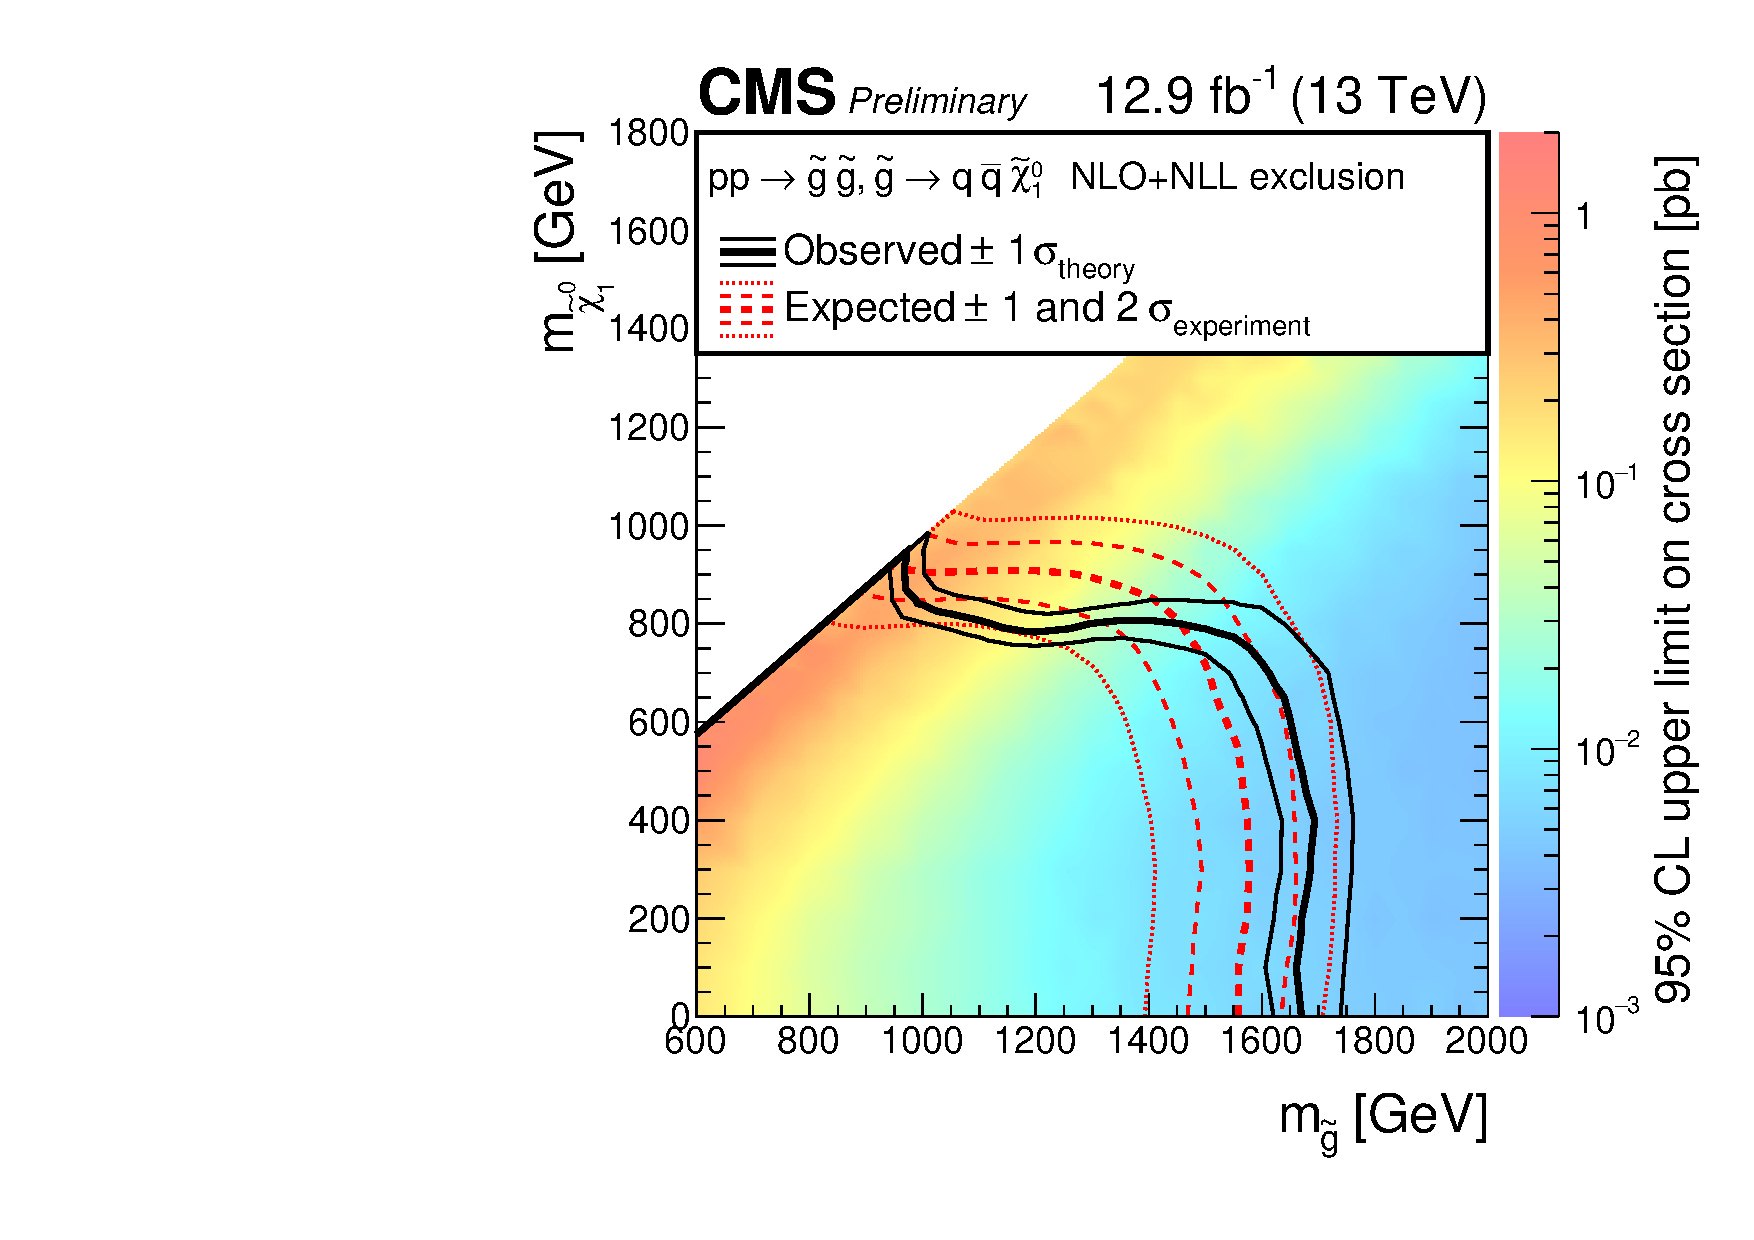
\includegraphics[width=0.49\textwidth]{SUS16T1qqqqXSEC.pdf} \\
    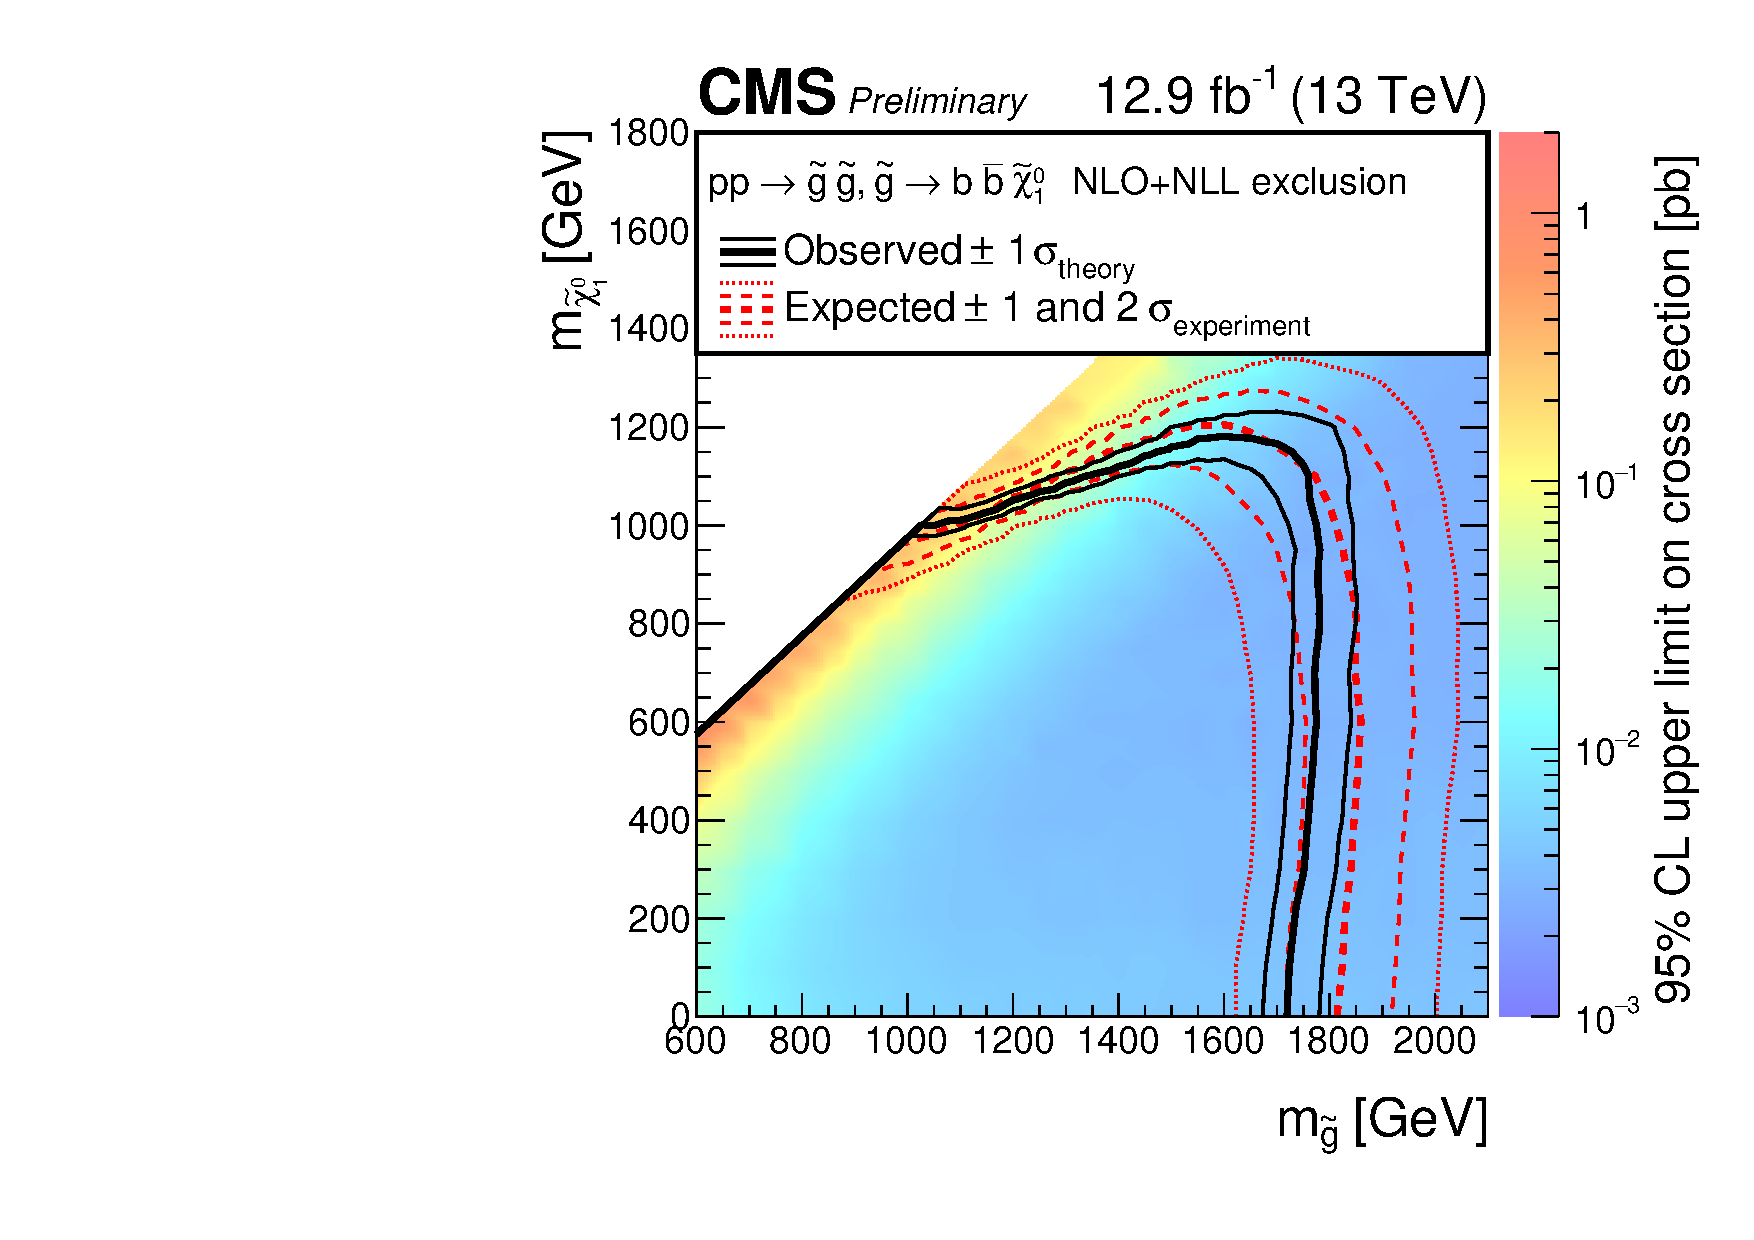
\includegraphics[width=0.49\textwidth]{SUS16T1bbbbXSEC.pdf} ~
    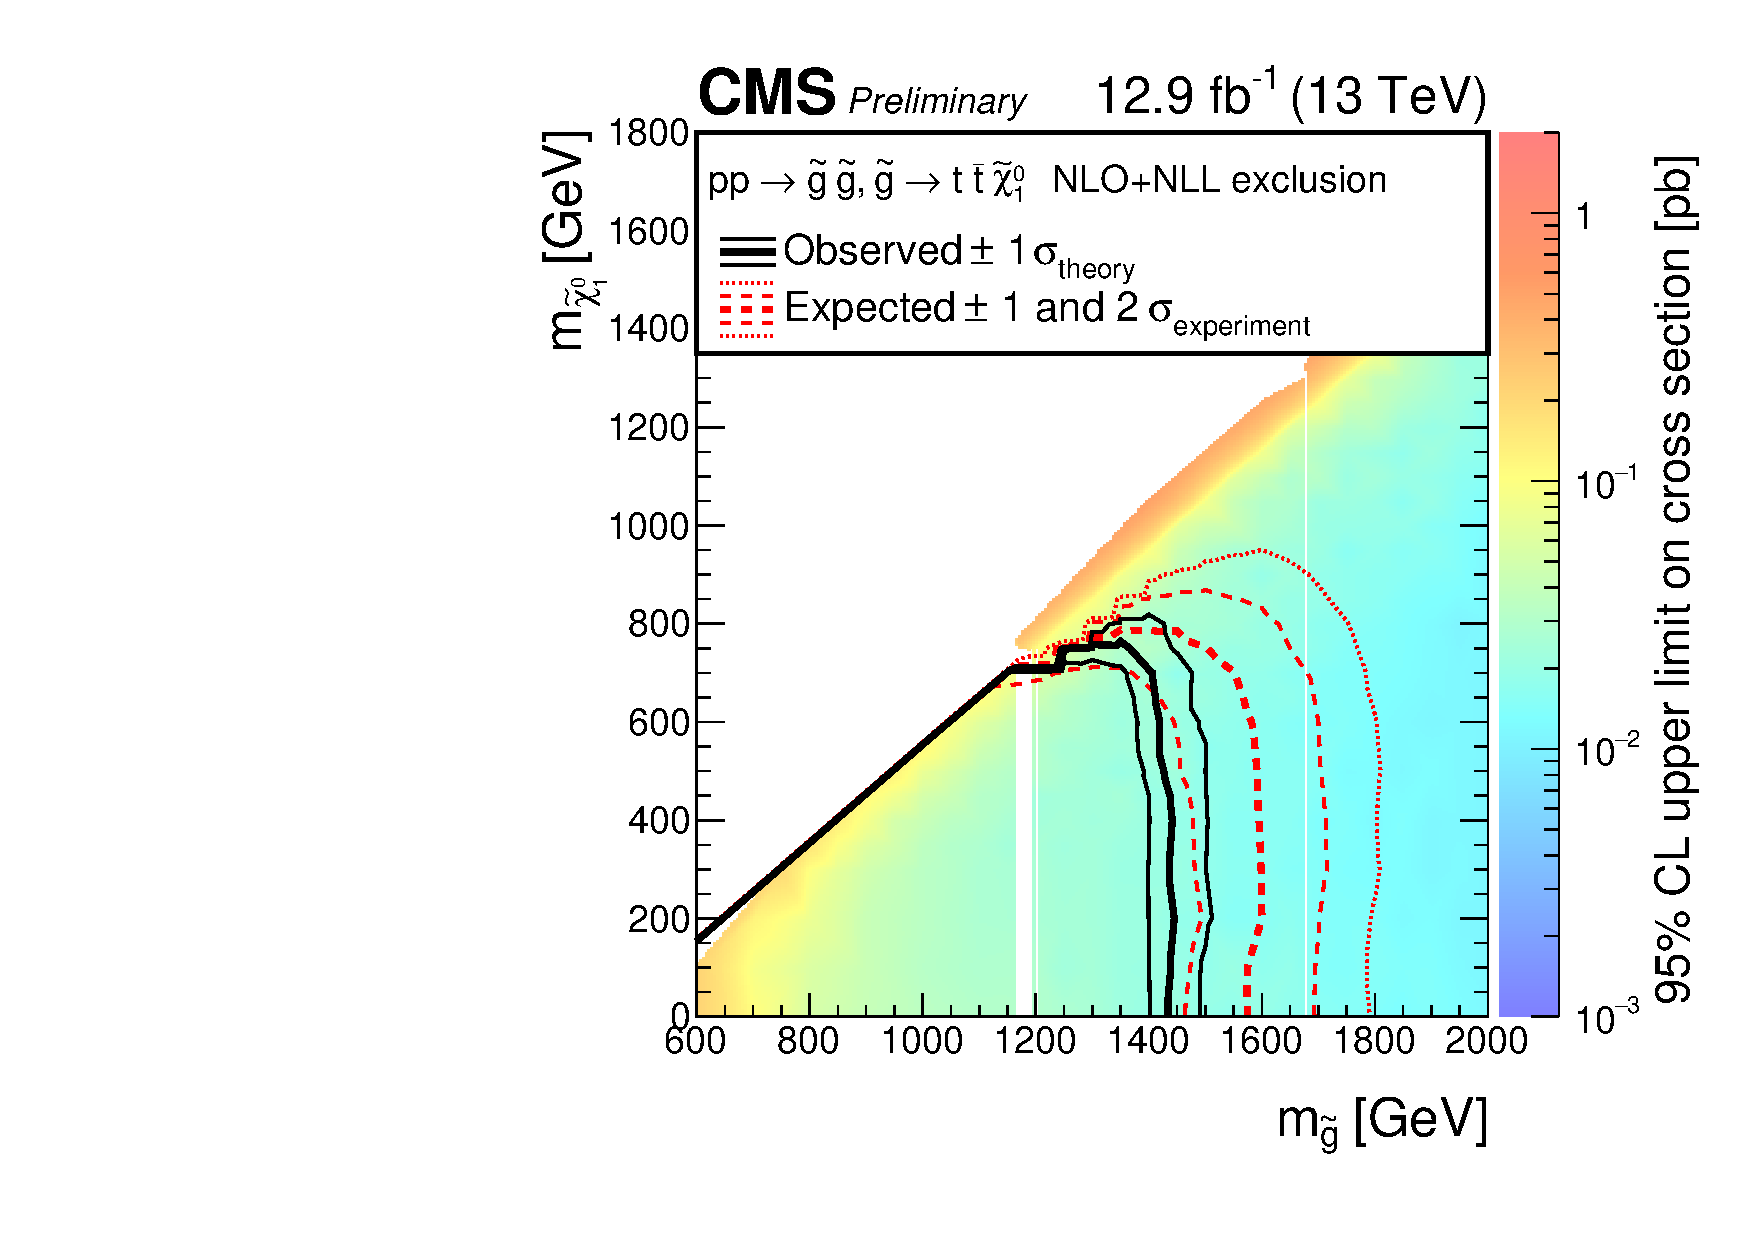
\includegraphics[width=0.49\textwidth]{SUS16T1ttttXSEC.pdf} 
    \caption{Observed upper limit in cross section at 95\% confidence
      level (indicated by the colour scale) for simplified models that
      assume the gluino-mediated production of (Top) light-flavour,
      (Bottom Left) bottom, and (Bottom Right) top squark pairs, as a
      function of the gluino or squark mass and the $\chiz_{1}$
      mass. The black solid thick (thin) line indicates the observed
      mass exclusion regions assuming the nominal (${\pm}1 \sigma$
      theory uncertainty) production cross section. The red dashed
      thick (thin) line indicates the median (${\pm}1 \sigma$
      experimental uncertainty) expected mass exclusion
      regions. 
      \label{fig:limits-sms-gluino} }
  \end{center}
\end{figure*}

\begin{figure*}[thp!]
  \begin{center}
    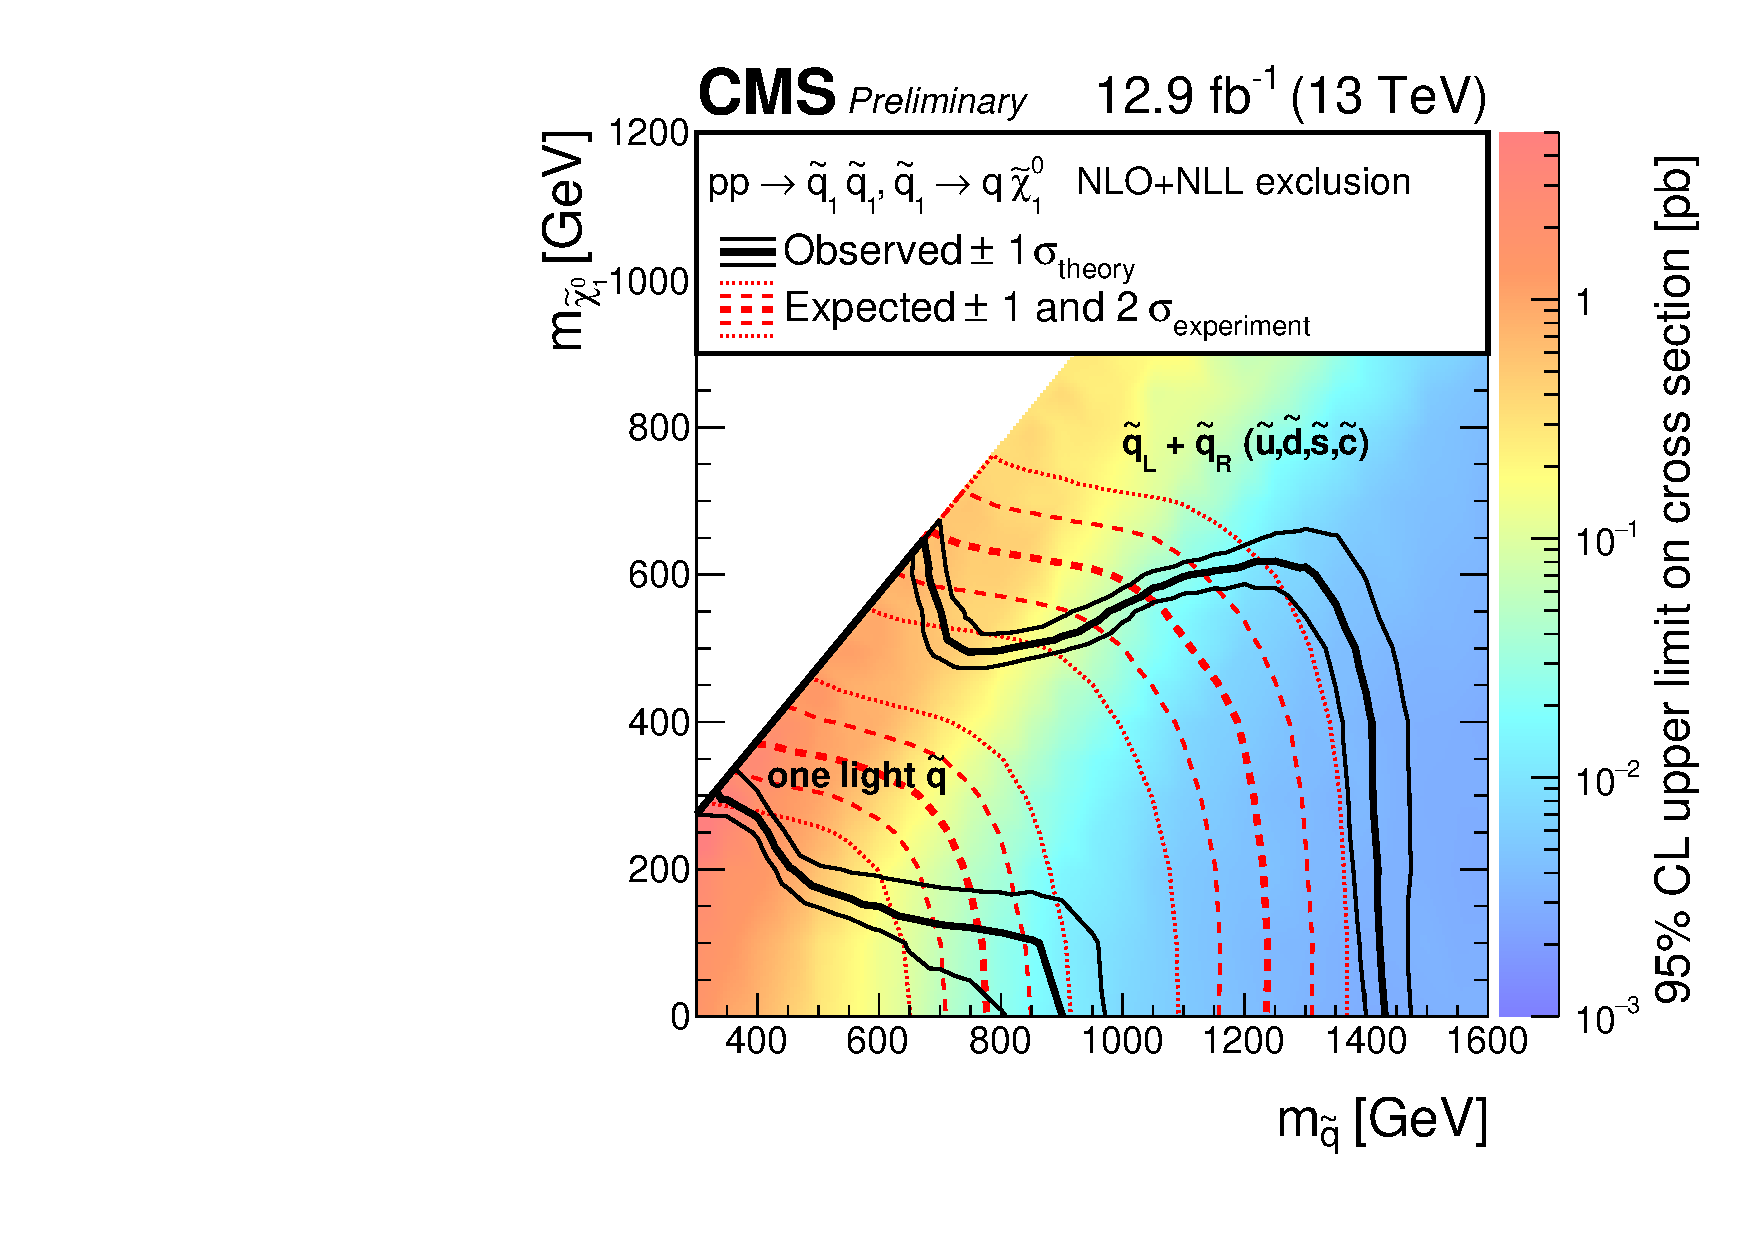
\includegraphics[width=0.49\textwidth]{SUS16T2qqXSEC.pdf} \\
    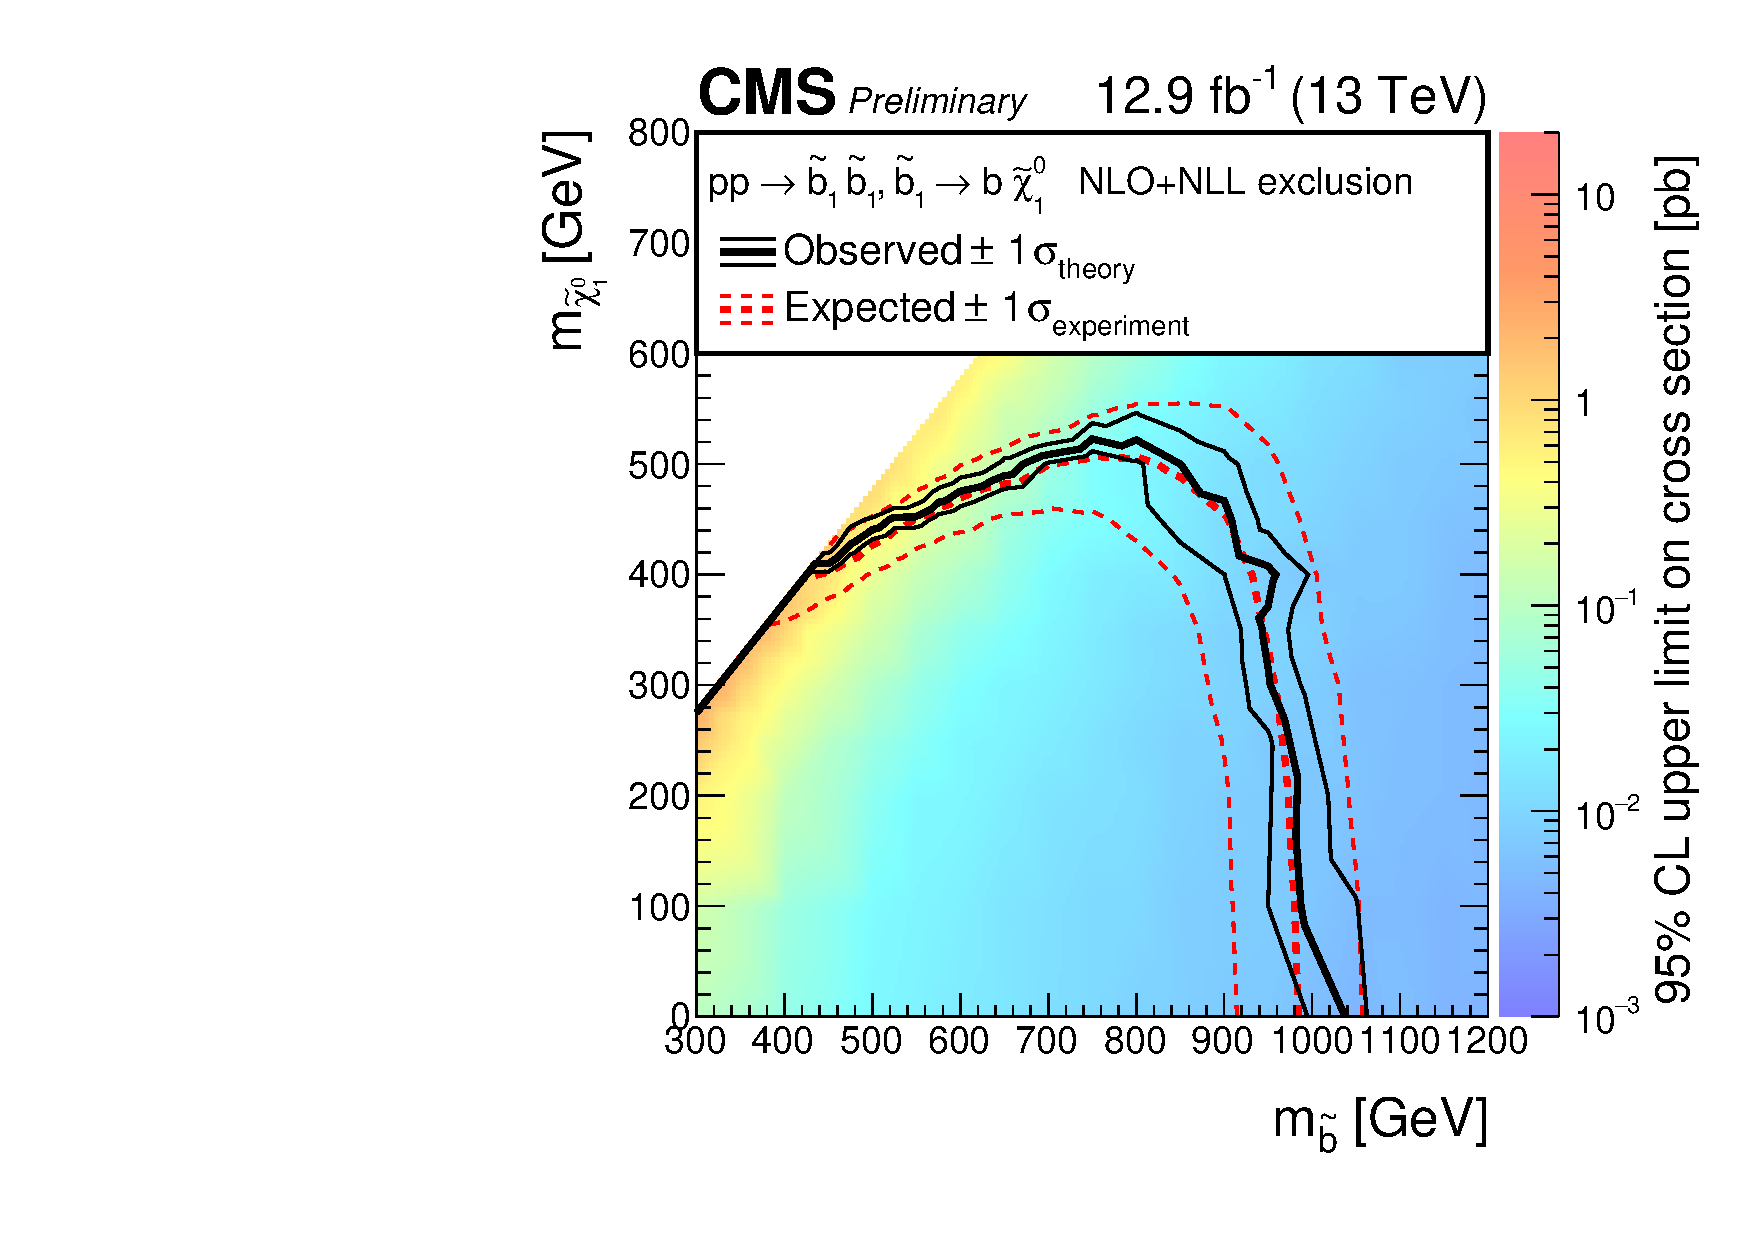
\includegraphics[width=0.49\textwidth]{SUS16T2bbXSEC.pdf} ~
    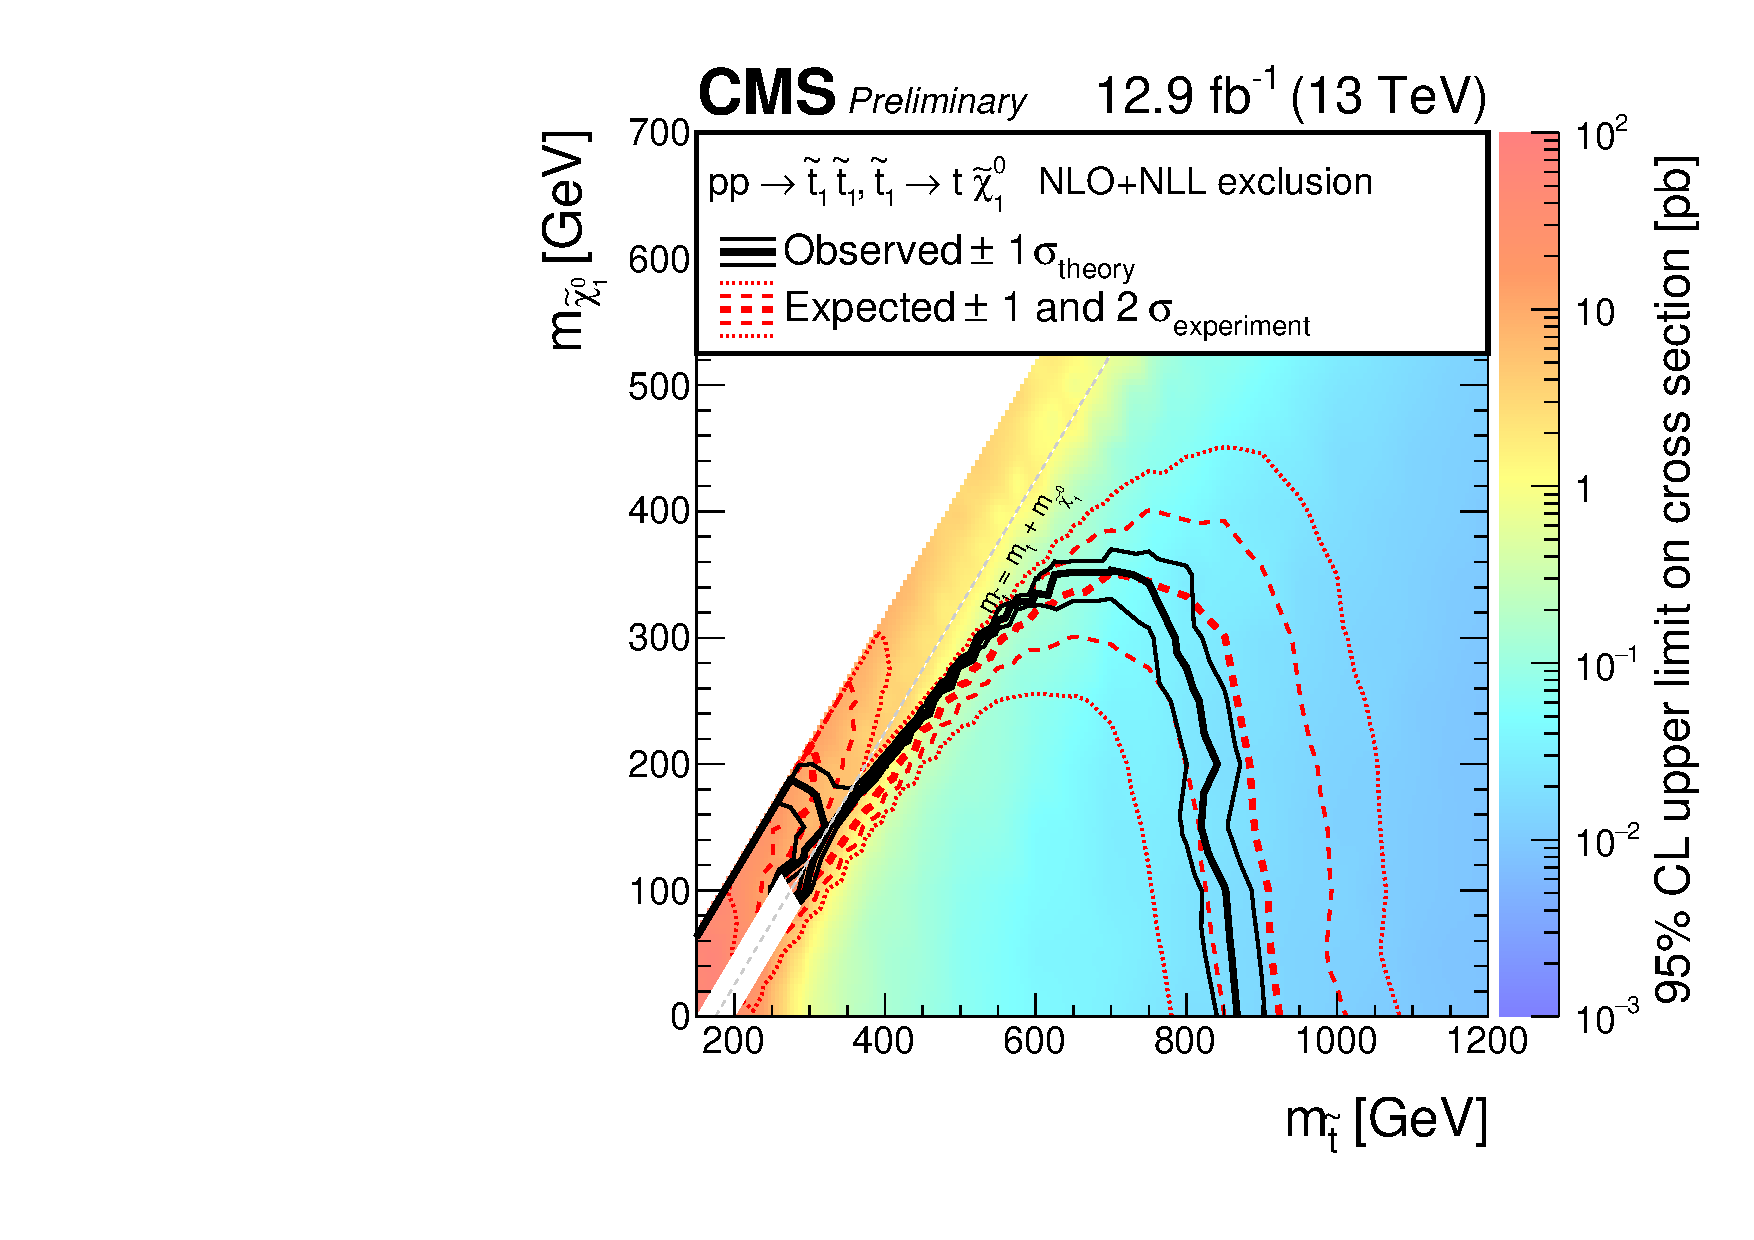
\includegraphics[width=0.49\textwidth]{SUS16T2ttXSEC.pdf} 
    \caption{Observed upper limit in cross section at 95\% confidence
      level (indicated by the colour scale) for simplified models that
      assume the direct production of (Top) light-flavour, (Bottom
      Left) bottom, and (Bottom Right) top squark pairs, as a function
      of the gluino or squark mass and the $\chiz_{1}$ mass. The black
      solid thick (thin) line indicates the observed mass exclusion
      regions assuming the nominal (${\pm}1 \sigma$ theory
      uncertainty) production cross section. The red dashed thick
      (thin) line indicates the median (${\pm}1 \sigma$ experimental
      uncertainty) expected mass exclusion regions. 
      \label{fig:limits-sms-squark} }
  \end{center}
\end{figure*}

Figure~\ref{fig:limits-sms-gluino} shows the observed upper limit on
the production cross section at 95\% confidence level as a function of
the gluino and \chiz masses for models that assume the gluino-mediated
production of light-flavour, bottom, and top squark pairs. Also shown
are the observed mass exclusion regions when varying the production
cross section by its theoretical uncertainty, and the expected mass
exclusion regions with the ${\pm}1$ and ${\pm}2$ standard-deviation
variations. Similarly, Figure~\ref{fig:limits-sms-squark} shows the
exclusion regions for models that assume the direct production of
light-flavour, bottom, and top squark pairs.

The search places stringent limits in the mass parameter space of
these models, with observed exclusions in gluino and \chiz masses as
high as 1775 and 1175\GeV, respectively. In the case of direct
production of light-flavour squarks, masses up to $\sim$1425 and
$\sim$650\GeV are excluded for the squark and \chiz, respectively,
when assuming an eightfold degeneracy in squark mass. These limits are
significantly weaker under the assumption of a single light
squark. Similarly, bottom squark and \chiz masses as high as
$\sim$1025 and $\sim$525\GeV are excluded. Finally, top squark and
\chiz masses up to $\sim$875 and $\sim$350\GeV are excluded. A summary
of the limits is provided in Table~\ref{tab:simplified-models-limits}.

\newcommand{\ph}{\ensuremath{\phantom{1}}}
\begin{table}[tb]
  \topcaption{Summary of the mass limits obtained for the six 
    classes of simplified models. ``Mass degeneracy'' refers to the
    number of mass-degenerate squarks that participate in the
    interaction. The limits indicate the strongest observed (expected)
    mass exclusions for the gluino or squarks, and $\chiz_1$, and the
    quoted values have uncertainties of $\pm$25\GeV. 
  }
  \label{tab:simplified-models-limits}
  \centering
  \footnotesize
  \begin{tabular}{ llccc }
    \hline
    Production mode & Squark        & Degeneracy & \multicolumn{2}{c}{Strongest obs. (exp.) mass exclusion [GeV]}\T\B \\
    \cline{4-5}                       
                    &               &            & Gluino or squark\T\B & \chiz                                               \\
    \hline                            
    Gluino-mediated & Light-flavour & -          & 1700 \ph(1575)       & \ph950 \ph\ph(900)                                  \\ 
    Gluino-mediated & Bottom        & -          & 1775 \ph(1850)       & 1175 \ph(1200)                                      \\ 
    Gluino-mediated & Top           & -          & 1450 \ph(1600)       & \ph750 \ph\ph(800)                                  \\ 
    Direct          & Light-flavour & 8          & 1425 \ph(1225)       & \ph650 \ph\ph(650)                                  \\ 
    Direct          & Light-flavour & 1          & \ph900 \ph\ph(775)   & \ph300 \ph\ph(375)                                  \\ 
    Direct          & Bottom        & 1          & 1025 \ph\ph(975)     & \ph525 \ph\ph(500)                                  \\ 
    Direct\B        & Top           & 1          & \ph875 \ph\ph(925)   & \ph350 \ph\ph(350)                                  \\
    \hline
 \end{tabular}
\end{table}

%%__________________________________________________________________||
